\documentclass[12pt, a4paper]{extarticle}
\usepackage[T1,T2A]{fontenc}
\usepackage[utf8]{inputenc}
\usepackage[russian]{babel}
\usepackage{tempora}

\usepackage[hidelinks]{hyperref}
\usepackage{amsmath}
\usepackage{amssymb}
\usepackage[paper=a4paper, left=35mm, right=10mm, bottom=15mm,top=15mm, includefoot]{geometry}
\usepackage{tocloft}
\usepackage{indentfirst}
\usepackage{fancyhdr}
\usepackage{titlesec}
\usepackage{tocloft}
\usepackage{booktabs}
\usepackage{chngcntr}
\usepackage{float}
\usepackage{tabularx}
\usepackage{graphicx}
\usepackage{float}
\usepackage{longtable}
\usepackage{svg}
\usepackage[justification=centering]{caption}
\captionsetup[table]{skip=10pt}

\counterwithin{figure}{section}
\counterwithin{table}{section}
\linespread{1.25}
\parindent=1.25cm
\addto\captionsrussian{\renewcommand*\contentsname{}}
\setlength\cftbeforesecskip{1pt}
\setlength\cftaftertoctitleskip{2.5mm}

\fancyhf{}
\fancyhead[C]{\thepage}
\fancyheadoffset{0mm}
\fancyfootoffset{0mm}
\renewcommand{\headrulewidth}{0pt}

\setlength{\headheight}{15mm}
\fancypagestyle{plain}{
    \fancyhf{}
    \chead{\thepage}}
\pagestyle{fancy}

\bibliographystyle{gost780s}


\renewcommand{\cfttoctitlefont}{\hfill\normalfont\normalsize\fontsize{14}{2.5mm}\bfseries Оглавление\hfill}
\renewcommand{\cftsecleader}{\cftdotfill{\cftdotsep}}
\newcommand*{\sectionformat}{\centering}

\titleformat*{\section}{\normalfont\fontsize{14}{2.5mm}\bfseries}
\titleformat*{\subsection}{\normalsize\bfseries}
\titleformat*{\subsubsection}{\normalsize\bfseries}

\renewcommand{\cftsecfont}{}
\renewcommand{\cftsecpagefont}{}




\begin{document}

  \begin{titlepage}
    \begin{center}
      \bfseries
      Федеральное государственное бюджетное образовательное учреждение высшего
      образования \\
      «МОСКОВСКИЙ ГОСУДАРСТВЕННЫЙ УНИВЕРСИТЕТ ИМЕНИ М. В. ЛОМОНОСОВА» \\
      ВЫСШАЯ ШКОЛА ГОСУДАРСТВЕННОГО АУДИТА\\
      НАПРАВЛЕНИЕ 38.03.01 ЭКОНОМИКА
    \end{center}
    \vspace{1cm}
    \begin{minipage}{5cm}
        Группа 305
    \end{minipage}
    \hfill
    \begin{minipage}{9cm}
      Кафедра государственных и \\муниципальных финансов
    \end{minipage}
    \vspace{70pt}
    \begin{center}
       \bfseries
       Реферат \\
       \large
       Оценка эффективности государственных расходов
    \end{center}
    \vspace{100pt}
    Студент-бакалавр \\
    Сергеев Владислав Александрович
    \hfill
    \begin{minipage}{7cm}
      {$/\_\_\_\_\_\_\_\_\_\_\_\_/\_\_\_\_\_\_\_\_\_\_\_\_/$}\\
      \phantom{8pt} (подпись) \hspace{40pt}(дата)
    \end{minipage}
    \\
    \vspace{10pt}
    \\
    \begin{minipage}{7.4cm}
      Научный руководитель
    \end{minipage}
    \\
    к.э.н., Ларионов Александр Витальевич
    \hfill
    \begin{minipage}{7cm}
      {$/\_\_\_\_\_\_\_\_\_\_\_\_/\_\_\_\_\_\_\_\_\_\_\_\_/$}\\
      \phantom{8pt} (подпись) \hspace{40pt}(дата)
    \end{minipage}
  \\
  \vspace{\fill}
  \begin{center}
    \bfseries\large
    Москва\\
    2022
  \end{center}


  \end{titlepage}
  \addtocounter{page}{1}

  % Оглавление
  \newpage
    \tableofcontents
  \newpage

  % Введение
  \section*{\sectionformat {Введение}}
  \addcontentsline{toc}{section}{Введение}
\par
    Одной из основных целей бюджетной реформы, проводимой в Российской Федерации начиная с 2004 года, является повышение эффективности расходов бюджетов бюджетной системы. В этой связи проводятся реструктуризация бюджетного сектора, реформа бюджетного процесса, изменяется механизм финансового обеспечения учреждений социальной сферы, что обусловливает необходимость уточнения теоретических и методических подходов к финансированию расходов бюджетов бюджетной системы на общее образование, оценке их эффективности с учетом современных требований к управлению государственными и муниципальными финансами.
\par
    Бюджетная политика является главным инструментом государственного регулирования экономики, она влияет на дальнейшее социально-экономическое развитие страны, поэтому важно знать, насколько бюджетная политика государства эффективна. Такая информация нужна для понимания того, насколько правильно реализуются экономические решения властей, применяются те или иные меры бюджетной политики. Для оценки эффективности государственных расходов стандартно используют значение мультипликатора государственных расходов.
\par
    \textbf{Цель данного исследования} -- анализ подходов оценивания эффективности государственных расходов. Для решения поставленной цели возникают следующие \textbf{задачи}:
  
  \begin{itemize}
    \renewcommand\labelitemi{--}
    \item Изучить методы вычисления мультипликаторов государственных расходов и их анализ в разных моделях;
    \item Выявить факторы, оказывающие влияние на эффективность расходов бюджетов и дать их классификационную характеристику;
    \item Расчитать мультипликаторы государственных расходов на основе российских данных
  \end{itemize}
\par
    \textbf{Объектом исследования} являются расходы бюджетов публично-правовых образований на общее образование. \textbf{Предметом исследования} являются институциональные особенности, бюджетная практика и методические аспекты оценки эффективности расходов бюджетов на оказание общеобразовательных услуг начального общего, основного общего, среднего общего образования.
\par
    В качестве информационной базы исследования были использованы официальные статистические данные и материалы Федеральной службы государственной статистики Российской Федерации; данные Федерального казначейства, Министерства финансов Российской Федерации, информационно-аналитические материалы ОЭСР, др.

\newpage
\section{Обзор литературы}

\par
    В экономике мультипликатор государственных расходов (фискальный мультипликатор) -- это отношение изменения национального дохода, возникающее в результате изменения государственных расходов. Существование эффекта мультипликатора было первоначально предложено студентом Кейнса Ричардом Каном в 1930 году и опубликовано в 1931 году.\cite{keyns} Некоторые другие школы экономической мысли отвергают или преуменьшают важность эффектов мультипликатора, особенно с точки зрения долгосрочной перспективы. Эффект мультипликатора использовался в качестве аргумента в пользу эффективности государственных расходов или налоговых льгот для стимулирования совокупного спроса.

\par
    Тема оценки фискальных мультипликаторов важна, поскольку центральные банки постепенно теряют способность стимулировать экономику путем снижения процентной ставки. Несмотря на важность, существует широкий диапазон различных оценок размера мультипликатора государственных расходов: то есть на сколько увеличивается совокупный объем производства в результате экзогенного увеличения государственных расходов. Знание мультипликаторов различных компонент позволяет выбрать оптимальную политику. В данной главе будут проведен литературный обзор оценки эффективности государственных расходов.
    
\subsection{Теоретические подходы к оценке мультипликатора}

\par
    При расчете валового внутреннего продукта (далее -- ВВП) используют сумму четырех компонентов: потребление ($C$), инвестиции ($I$), государственные расходы ($G$) и чистый экспорт ($Nx$):


\begin{equation}
    Y = C + I + G + Nx, 
    \label{eq: GDP}
\end{equation}

где $Y$ -- ВВП (Gross Domestic Product, GDP)


\par
    Активное использование бюджетной политики в период мирового финансового кризиса 2008—2009 гг. породило новую волну научных дискуссий о ее возможностях и эффективности. Основной вопрос: какое влияние оказывает увеличение госрасходов сегодня на выпуск в будущем? В экономике данный эффект количественно измеряется при расчете мультипликатора государственных расходов, показывающий влияние дискреционного изменения основных бюджетных показателей (расходов – $\Delta FI$) в периоде $t$ на изменение ВВП ($\Delta Y$) на горизонте $i$:


\begin{equation}
    i = \frac{\Delta Y(t + i)}{\Delta FI}
\end{equation}


\par
    В экономической теории используются два подхода к определению мультипликатора. Во-первых, мультипликатором называется совокупный прирост одного показателя в результате единичного прироста другого. Во-вторых, под мультипликатором можно понимать текущий прирост показателя как результат единичного прироста его фактора в каждом из прошедших периодов. Оба подхода на примере процесса инвестирования в основой капитал рассматриваются в статье Пола Самуэльсона.\cite{samuelson}

\par
    В экономических исследованиях наблюдается явный перекос в пользу мультипликатора первого типа. Разработанные и опробованные на реальных данных методики расчета мультипликатора ориентированы именно на оценку отклика ВВП на единичный шок показателя бюджетной политики. 

\par
    Для принятия решений в рамках бюджетной экономической политики более важным является показатель реакции экономики (в частности, ВВП) на единичное приращение государственных закупок в среднем, поскольку данный показатель позволяет построить прогноз динамики ВВП и прочих, не менее важных экономических переменных.

\par
    Суммарный эффект от роста госрасходов для ВВП зависит от величины всех эффектов для спроса и предложения товаров и услуг. Увеличение госрасходов непосредственно ведет к росту спроса. Но это прямое влияние на спрос компенсируется уменьшением других его составляющих. Со стороны предложения количество эффективных часов может как увеличиться, так и уменьшиться. Чтобы уравнять спрос и предложение товаров и услуг, в модели обычно присутствует переменная, которая свободно подстраивается под изменившиеся условия в экономике. Обычно это реальная или номинальная процентная ставка. Из обзора теоретических моделей \cite{ramey} следует, что в теории можно получить достаточно широкий диапазон значений мультипликатора в зависимости от того, за счет каких средств финансируются госрасходы, и других факторов. К сожалению, этот диапазон значений такой широкий, что нельзя однозначно сказать, приведет увеличение госрасходов к росту ВВП или нет.
    
\subsection{Эмпирические оценки фискального мультипликатора}

\par
    Из обзора теоретических моделей \cite{ramey} следует, что в теории можно получить достаточно широкий диапазон значений мультипликатора в зависимости от того, за счет каких средств финансируются госрасходы, и других факторов. К сожалению, этот диапазон значений такой широкий, что нельзя однозначно сказать, приведет увеличение госрасходов к росту ВВП или нет.

\par
    Так в статье Кудрина и Кнобеля \cite{kudrin} описывается проблема причинности модели: корреляция между динамикой госрасходов и ВВП не позволяет однозначно утверждать, что рост ВВП связан с ростом госрасходов, так как может иметь место противоположная ситуация. Обойти проблему причинности можно через фокусирование оценки эффективности бюджетных расходов на функциональных разделах и направлениях финансирования, о которых априори известно, что они не подвержены изменениям вслед за динамикой ВВП. В этой же статье \cite{kudrin} применяют идентификационные рекурсивные ограничения, основанные на оценки модели SVAR (Structural Vector Autoregression), которая в матричном виде выглядит как \ref{eq:svar}:
    
\begin{equation}
    A Z_{t}=A_{0}+C(L) Z_{t-1}+e_{t},
    \label{eq:svar}
\end{equation}
    
где $Z_{t}$ – вектор эндогенных переменных размерностью $k$, наблюдаемых в период времени $t$; $e_{t}$ – вектор структурных шоков размерностью $k$, наблюдаемых в период времени $t$, $e_{t} \sim\left(0, \Sigma_{e}\right)$; $A_{0}$ – вектор констант размерностью $k$; $A$ – матрица коэффициентов размерно- стью $k \times k$; $C(L)$ – лаговый оператор порядка $p$.

\par
    В целом, подходы к эмпирическому оцениванию фискального мультипликатора можно разделить на два основных: структурные векторные авторегрессии (SVAR) и модели общего стохастического равновесия (Dynamic Stochastic General Equilibrium modeling, DSGE), которую в общем виде можно записать как \ref{eq:dsge}:
    
\begin{equation}
    \left[\begin{array}{c}
    X_{t+1} \\
    H x_{t+1 \mid t}
    \end{array}\right]=A\left[\begin{array}{c}
    X_{t} \\
    x_{t}
    \end{array}\right]+B i_{t}+\left[\begin{array}{c}
    C \\
    0
    \end{array}\right] \varepsilon_{t+1}
    \label{eq:dsge}
\end{equation}

\par
    Проблема эндогенности, описанная выше, встречается во многих исследованиях (\cite{blanchard}, \cite{favero}). Определение шоков фискальной политики стало главным отличием в исследованиях, основанных на векторных авторегрессиях (VAR). Так, выделяют "технический" (technical) и "нарративный" (narrative) подходы. При техническом подходе шоки бюджетной политики -- это остатки SVAR-модели; при нарративном подходе шоки получаются отдельным расчетом, отличным от модели, используемой для оценки мультипликаторов. Таким образом, при нарративном подходе сначала оцениваются шоки государственных доходов или расходов, затем готовые ряды шоков подставляются в качестве переменной в основную модель, с помощью которой оцениваются мультипликаторы. Большинство работ по фискальным мультипликаторам используют структурные SVAR-модели с технической идентификацией, а также совмещают ее с внешней информацией, по примеру того, как это сделано в работе Бланшара и Перотти \cite{blanchard}.
    
    
\par
    В России существует проблема отсутствия длинных, сопоставимых рядов данных по многим показателям, что объясняется отличием стандартов советской и мировой статистики и продолжающимся переходом официальных органов к новым методикам расчета, часто без соответствующей переоценки предыдущих значений. Среди российских работ можно выделить исследование Ивановой и Каменских \cite{ivanova}, в котором анализируется эффективность госрасходов в России в 2000—2010 гг. Авторы рассчитали как общий мультипликатор для совокупного объема госрасходов, так и отдельные мультипликаторы для функциональных разделов госрасходов. Для получения значений мультипликаторов используется двухшаговая процедура.
    
\par
     Российские исследования фискальных мультипликаторов дают достаточно большой разброс оценок как по расходам (от 0,13 до 0,91), так и по доходам (от –0,75 до –0,10).


\subsection*{{Выводы}}
\addcontentsline{toc}{subsection}{Выводы}

\par
    VAR-модели показывают "средний" отклик ВВП на шоки бюджетной политики, и мультипликаторы, полученные с их помощью, как правило, используются, когда состояние экономики близко к "нормальному". Когда состояние экономики существенно отличается от нормального, более эффективными могут оказаться оценки, полученные с помощью DSGE-моделей, если они хорошо отражают текущие характеристики экономики. Обзор DSGE-моделей представлен в работе \cite{dsge}.

\par
    Также используются более редкие подходы для оценки фискальных мультипликаторов: байесовские SVAR \cite{cb}, векторные модели коррекции ошибок  (VECMX) \cite{belarus}.



\newpage
\section{Методика оценивания и данные}

В данной главе будут описаны данные, которые были отобраны для построения модели для оценивания фискального мультипликатора. Будет эконометрический  анализ представлений данных при помощи модели SVAR. Это некоторая модификация классического метода векторной авторегрессии (VAR) и отличается от последнего тем, что накладывает дополнительные ограничения на матрицы коэффициентов. В настоящее время этот метод считается наиболее популярным инструментом оценки фискальных мультипликаторов.

\subsection{Описание данных}
\par
    Фискальные мультипликаторы для совокупных бюджетных расходов ($GM$) консолидированного бюджета РФ оцениваются на квартальных данных: с первого квартала 2013 по третий квартал 2021 года. Помимо показателя квартального ВВП в постоянных ценах 2016 года ($Y$) в рассматриваемой в работе модели используется показатель номинальной ключевой ставки ($i$) Банка России в качестве показателя монетарных условий и налоговые доходы бюджета ($T$) . В качестве экзогенных переменных -- цена на нефть марки Urals ($P_{oil}$), нефтегазовые ($I_{oil}$) доходы бюджета и ключевая ставка ЦБ РФ ($i$). Источниками данных являются  Росстат, информационные агентства, сайт Министерства Финансов РФ.
    Включение в уравнения переменных цены на нефть и объема нефтегазовых доходов объясняется сохраняющейся зависимостью от нефтегазовой отрасли российской экономики в целом и доходов федерального бюджета в частности.

\par
    Все показатели приведены в реальное выражение с помощью индекса-дефлятора ВВП (кроме номинальной процентной ставки и цены на нефть) и представлены в виде натуральных логарифмов (за исключением номинальной процентной ставки).

\par
    На \figurename{\ref{fig:spends_gpd}} представлена динамика расходов бюджета (в \% ВВП) по отдельным разделам за 2013—2019 гг. За исключением расходов на ЖКХ, расходы по различным разделам сильно коррелируют между собой: одновременно падают или растут в зависимости от уменьшения или увеличения общих расходов бюджета.
    
\begin{figure}[H]
  \caption{Расходы бюджета по функциональным разделам (\% ВВП)}
  \centering
  \noindent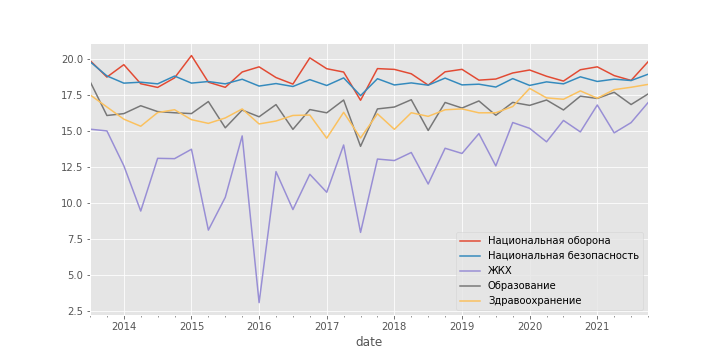
\includegraphics[scale=0.5]{spends.png}
  \label{fig:spends_gpd}
\end{figure}

\subsection{Описание модели}


Чтобы оценить мультипликаторы расходов для рассматриваемых разделов бюджетной классификации, предположим, что экономическая система России описывается моделью из трех одновременных уравнений: определяющего расходы бюджета, определяющего доходы и определяющего ВВП. При этом в модели все переменные по умолчанию эндогенные. Соответственно для оценки этой динамической системы необходимо сделать дополнительные предположения, например о том, что некоторые переменные экзогенные по отношению к другим, исходя из их экономического смысла. Предположим, во-первых, что цена на нефть на мировом рынке, нефтегазовые доходы и ключевая ставка заданы экзогенно; во-вторых, что расходы бюджета в текущем периоде не зависят от ВВП того же периода. Таким образом, рассматриваемая модель для оценки мультипликаторов бюджетных расходов имеет следующий вид:

\begin{equation}
    \resizebox{.93\hsize}{!}{
    \left(\begin{array}{c}
    ln T_{t} \\
    ln G_{i, t} \\
    ln Y_{t}
    \end{array}\right)=\left(\begin{array}{c}
    \delta_{T} \\
    \delta_{G_{i}} \\
    \delta_{Y}
    \end{array}\right)+\sum_{j=1}^{k} B_{j}\left(\begin{array}{c}
    ln T_{t-j} \\
    ln G_{i, t-j} \\
    ln  Y_{t-j}
    \end{array}\right)+\left(\begin{array}{c}
    \gamma_{T_{i}} \\
    \gamma_{G_{i}} \\
    \gamma_{Y}
    \end{array}\right) \ln P_{oil, t}+\left(\begin{array}{c}
    \psi_{T_{i}} \\
    \psi_{G_{i}} \\
    \psi_{Y}
    \end{array}\right) i_{t}+\left(\begin{array}{c}
    \alpha_{T_{i}} \\
    \alpha_{G_{i}} \\
    \alpha_{Y}
    \end{array}\right) \ln I_{oil, t}+\left(\begin{array}{ccc}
    1 & 0 & 0 \\
    a_{21} & 1 & 0 \\
    a_{31} & a_{32} & 1
    \end{array}\right)\left(\begin{array}{c}
    e_{T, t} \\
    e_{G_{i, t}} \\
    e_{Y, t}
    \end{array}\right)},
    \label{eq:model}
\end{equation}

где $e$ — структурные шоки соответствующих переменных. Для нас наибольший интерес представляет коэффициент $a_{32}$, который отражает реакцию ВВП на единичный шок бюджетных расходов в текущем периоде. Если произойдет независимое увеличение логарифма расходов на 1, то в ответ на это логарифм ВВП увеличится на величину $a_{32}$.


\subsection{Эмпирические результаты}
\par
В рамках модели, представленной в формуле (\ref{eq:model}), рассматриваются два вида шоков: шок совокупных государственных доходов и шок совокупных государственных расходов. Интерес представляет только шок госрасходов ($a_{32}$)
\par
Итоговая модель оценивалась на различных количествах лагов. Выбор был сделан на основании критерия Акаике (AIC). Было выбрано два лага (значение критерия Акаике -- $-26.52$) Мы приводим оценки только коэффициента $a_{32}$, который интерпретируем как мультипликатор бюджетных расходов по ВВП. Результаты оценок этого мультипликатора в SVAR-модели с двумя лагами (именно модель с таким количеством лагов была выбрана на основе информационных критериев) представлены в таблице \ref{table:result}. Графики импульсных откликов (\figurename{\ref{fig:response}}) показывают, что есть статистически значимые отклики. Тесты на причинность по Грейнджеру показывают (\tablename {\ref{table:granger}}), что есть коинтеграция между некоторыми рядами при критическом p-значении 0.05:

\begin{table}[ht]
  \caption{Коинтеграция}
  \centering
  \begin{tabular}{|c|c|}
    \toprule
    Переменная & p-значение \\
    \midrule
    Национальная оборона & 0.015 \\ \hline
    Национальная безопасность & 0.507\\ \hline
    ЖКХ &  0.009 \\ \hline
    Образование & 0.269 \\ \hline
    Здравоохранение & 0.967 \\ \hline
  \end{tabular}
  \label{table:granger}
\end{table}


\begin{table}[ht]
  \caption{Результаты моделирования}
  \centering
  \begin{tabular}{|c|c|}
    \toprule
    Переменная & Значение мультипликатора \\
    \midrule
    Национальная оборона & 1.101 \\ \hline
    Национальная безопасность & 1.108\\ \hline
    ЖКХ &  1.047 \\ \hline
    Образование & 1.064 \\ \hline
    Здравоохранение & 1.071 \\ \hline
  \end{tabular}
  \label{table:result}
\end{table}


\begin{figure}[H]
  \caption{Импульсные отклики}
  \centering
  \noindent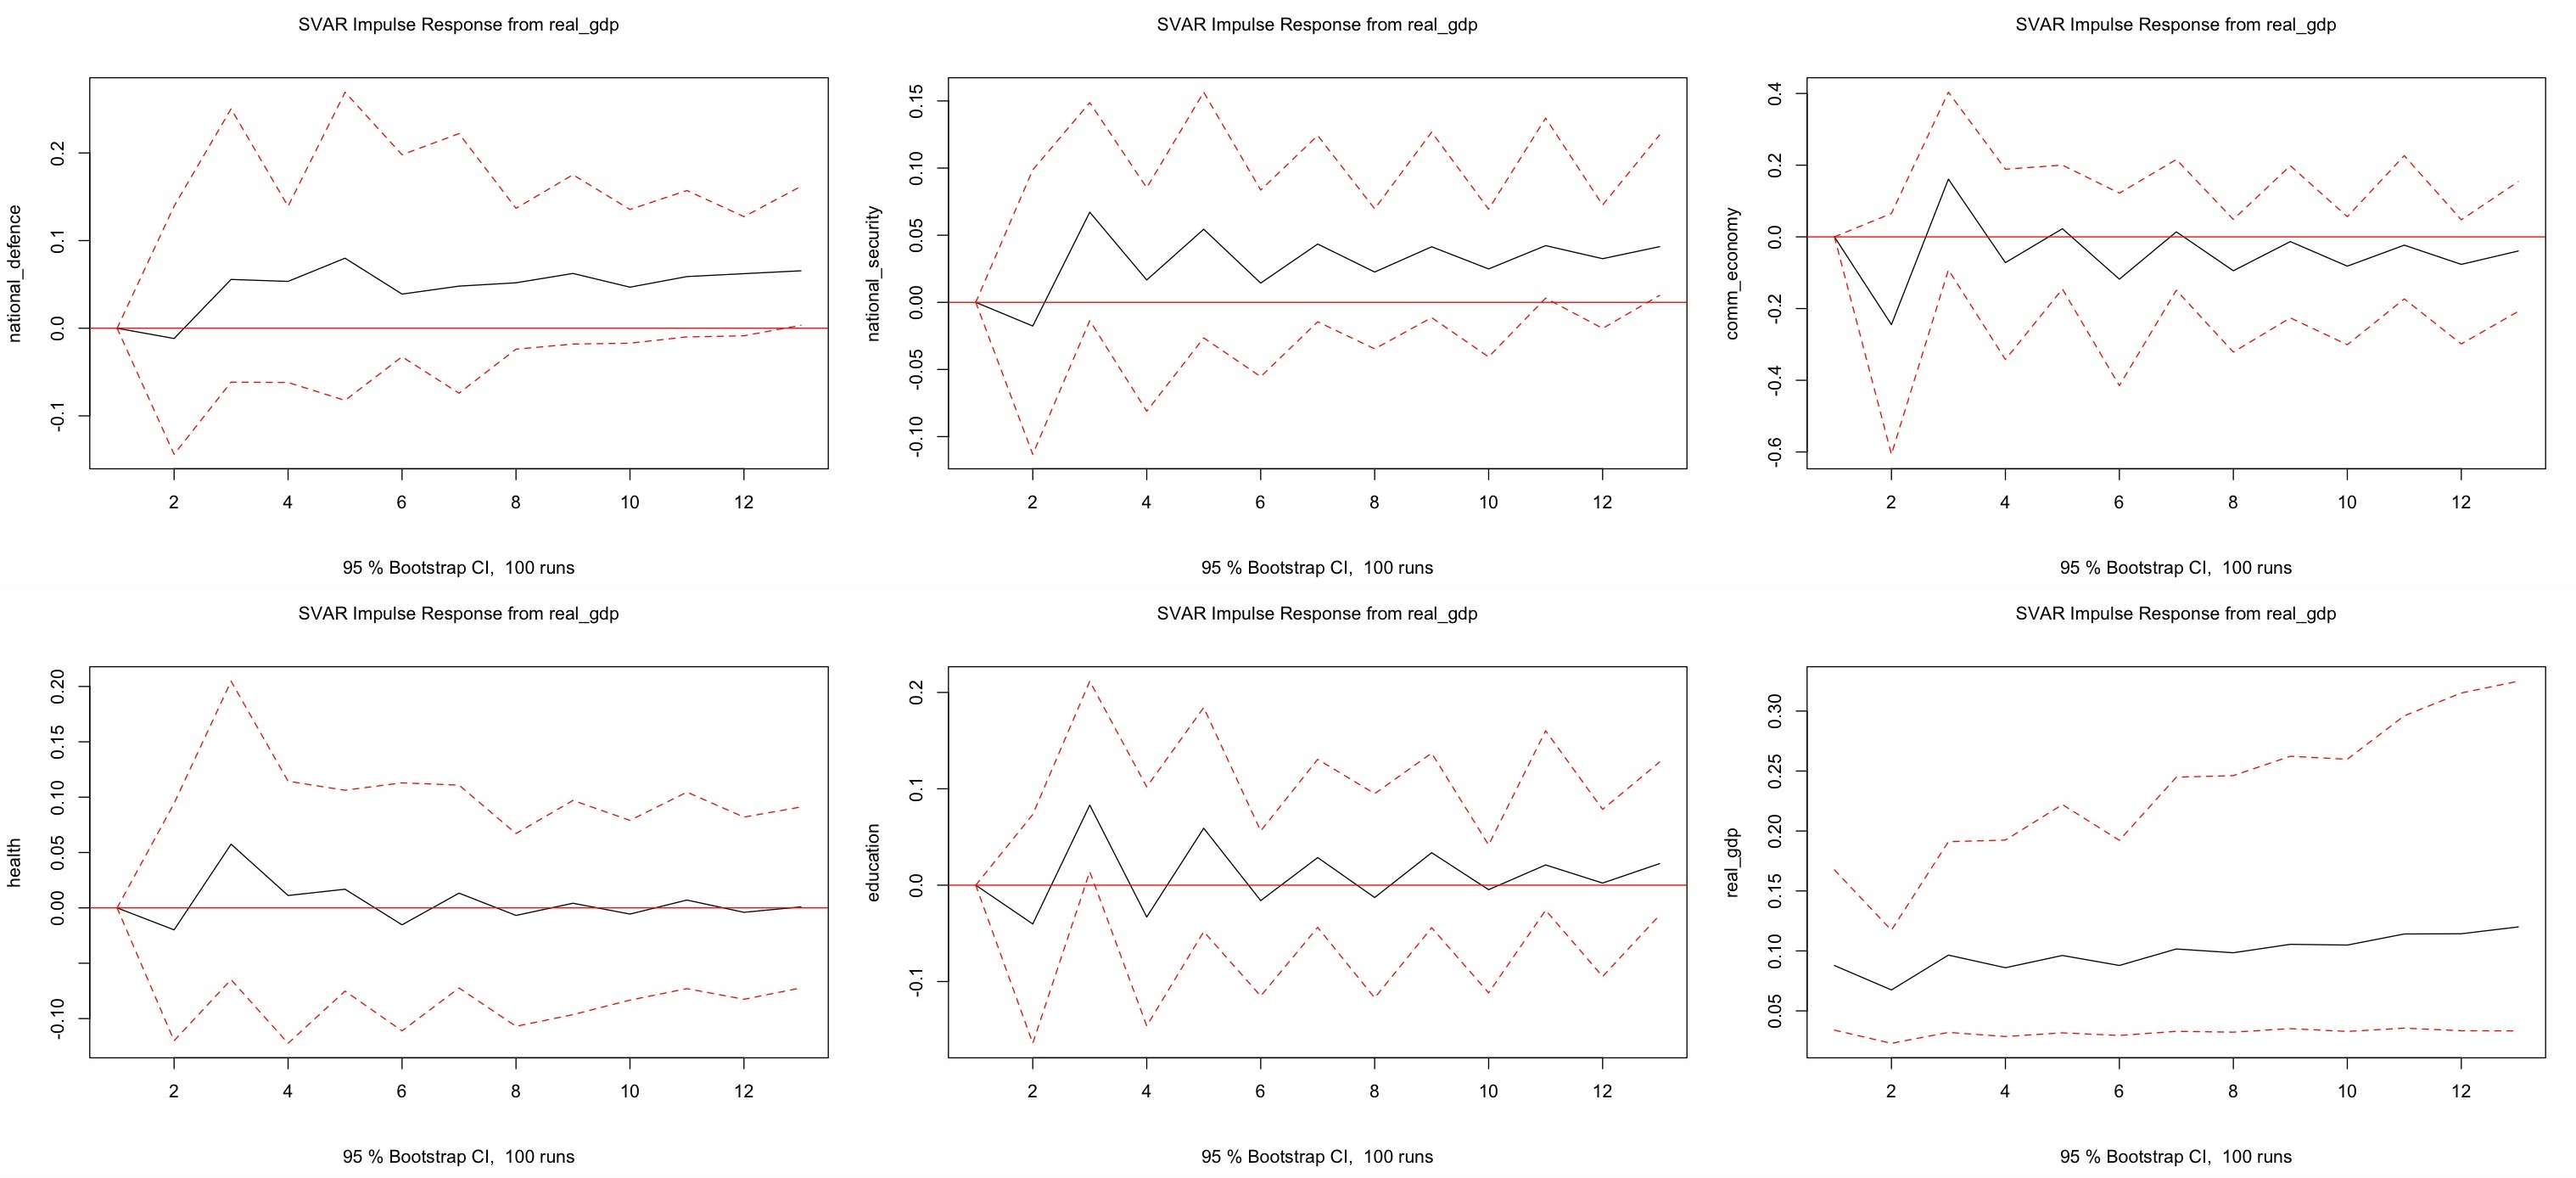
\includegraphics[width=\linewidth]{response.jpg}
  \label{fig:response}
\end{figure}


\subsection*{{Выводы}}
\addcontentsline{toc}{subsection}{Выводы}

Шоки статистически значимы. В целом можно заключить, что полученные результаты согласуются со значениями мультипликаторов бюджетных расходов для Российской Федерации в других работах.

\newpage
\section*{\sectionformat {Заключение}}
\addcontentsline{toc}{section}{Заключение}

\par
В работе произведена оценка эффективности структуры бюджетных расходов на экономику. Для этого были оценены фискальные мультипликаторы уровня ВВП по различным  направлениям расходов бюджета. В данной работе оценки мультипликаторов расходов по различным функциональным разделам бюджетной классификации проводились с помощью модели векторной авторегрессии. Этот подход основан на оценке системы уравнений, где каждая переменная зависит от лагов всех переменных системы. Так как при таком подходе все переменные системы эндогенные, то влияние одной переменной на другую оценивается через ответную реакцию переменной на изменение другой переменной.
\par
Полученные нами оценки устойчивы к изменению набора переменных, включенных в модель, в частности к использованию цены нефти в долларовом выражении. 
Представленные данные свидетельствует также о том, что реализация фискальной и денежно-кредитной политики в РФ были сориентированы на достижение одной цели -- рост ВВП вне зависимости от динамики экономического циклаи. Как следствие, рост госдоходов мог сопровождаться снижением ключевой ставки, несмотря на риск роста инфляционных процессов в экономике. С целью повышения эффективности реализации макроэкономической политики целесообразно повысить скоординированность применения инструментов макроэкономического регулирования в соответствии с динамикой экономического цикла. Это позволит усилить стратегический характер макроэкономической политики, нацеленный на поддержание устойчивых темпов экономического роста в долгосрочной перспективе.


\newpage
\addcontentsline{toc}{section}{Список литературы}
\titleformat*{\section}{\bfseries\normalsize\fontsize{14}{2.5mm}\centering}
\begin{thebibliography}{3}
    

    \bibitem{kudrin}
      Кудрин А., Кнобель А. (2017). Бюджетная политика как источник экономического роста // Вопросы экономики. No 10. С. 5—26. [Fiscal policy as a source of economic growth. Voprosy Ekonomiki, No. 10, pp. 5—26. (In Russian).]
      
    \bibitem{cb}
        Власов С.А., Дерюгина Е.Б. Фискальные мультипликаторы в России // Банк России: Серия докладов об экономических исследованиях. 2018. No 28. С. 1–19.
    
    \bibitem{ivanova}
        Иванова Н., Каменских М. (2011). Эффективность государственных расходов в Рос- сии // Экономическая политика. No 1. С. 176—192. [Ivanova N., Kamenskikh M. (2011). Budget expenditures effectiveness in Russia. Ekonomicheskaya Politika, No. 1, pp. 176—192. (In Russian).]
        
    \bibitem{belarus}
         О.Мазоль Оценка фискальных мультипликаторов для экономики Беларуси // Belarusian Economic Research and Outreach Center, Working Paper Series WP No. 65
      
    \bibitem{keyns}
    Snowdon, Brian; Vane, Howard R. (2005). Modern macroeconomics: its origins, development and current state. Edward Elgar. p. 61. ISBN 978-1-84542-208-0.
    
    \bibitem{samuelson}
    Samuelson P.A., A fundamental multiplier identity, Econometrica, Vol. 11, No 3⁄4 (Jul.-Oct., 1943), pp. 221-226
    
    \bibitem{ramey}
    Ramey V. A. (2011). Can government purchases stimulate the economy? Journal of Economic Literature, Vol. 49, No. 3, pp. 73—85.
    
    \bibitem{blanchard}
    Blanchard O., Perotti R. (2002) An Empirical Characterization of the Dynamic Effects of Changes in Government Spending and Taxes on Output. The Quarterly Journal of Economics, 117, pp. 1329–1368.
    
    \bibitem{favero}
    Favero C., Giavazzi F. (2012). Measuring Tax Multipliers: The Narrative Method in Fiscal VARs // American Economic Journal: Economic Policy, Vol. 4, No. 2, pp. 69–94.
    
    \bibitem{dsge}
        Coenen G., Erceg C.J., Freedman C., Furceri D., Kumhof M., Lalonde R., Laxton D., Lindé J., Mourougane A., Muir D., Mursula S., de Resende C., Roberts J., Roeger W., Snudden S., Trabandt M., Veld J. (2012). Effects of Fiscal Stimulus in Structural Models // American Economic Journal: Macroeconomics, Vol. 4, No. 1, pp. 22–68.




\end{thebibliography}

\end{document}
